\newpage	
{\samepage	
\begin{center}	
{\Large{\bf Binary Trees}}	
\end{center}	
\begin{itemize}	
\item Binary trees are used extensively in computer science	
\item Game Trees	
\item Searching	
\item Sorting	
\end{itemize}	
\begin{center}	
\includegraphics[width=\textwidth]{../Images/Linkedb.pdf}	
\end{center}	
}	

\newpage	
{\samepage	
\begin{center}	
{\Large{\bf Nomenclature}}	
\end{center}	
\begin{itemize}	
\item Trees drawn upside-down !	
\item Ancestor relationships: A is the parent of E	
\item Can refer to left and right children	
\item In a tree, there is only one path from the root to any child	
\item A node with no children is a leaf	
\item Most trees need to be created dynamically	
\item Empty subtrees are set to NULL	
\end{itemize}	
\begin{verbatim}	
typedef struct Node {	
   char letter;	
   struct Node *left;	
   struct Node *right;	
}	
\end{verbatim}	
}	

\newpage	
{\samepage	
\begin{center}	
{\Large{\bf Binary Trees\\[1.75ex]{\small(via an Array)}}}	
\end{center}	
Don't rush to assume a linked data structure must be used to implement	
trees. You could use $1$ cell of an array for the first node, the next	
two cells for its children, the next $4$ cells for their children and	
so on. You need to mark which cells are in use \& which aren't ...	
Counting from cell $1$:	

\begin{center}	
\begin{tabular}{|l|l|l|}\hline	
To find & Use & Iff\\ \hline	
The root & $A[1]$ & $A$ is nonempty \\	
The left child of $A[i]$ & $A[2i]$ & $2i \leq n$ \\	
The parent of $A[i]$ & $A[i/2]$ & $i > 1$\\	
Is $A[i]$ a leaf ? & True & $2i > n$\\ \hline	
\end{tabular}	
\end{center}	
}	



\newpage	
{\samepage	
\begin{center}	
{\Large{\bf Binary Search Trees}}	
\end{center}	
In a binary search tree the left-hand tree of a parent contains all keys less than the parent node,	
and the right-hand side all the keys greater than the parent node.	
\begin{center}	
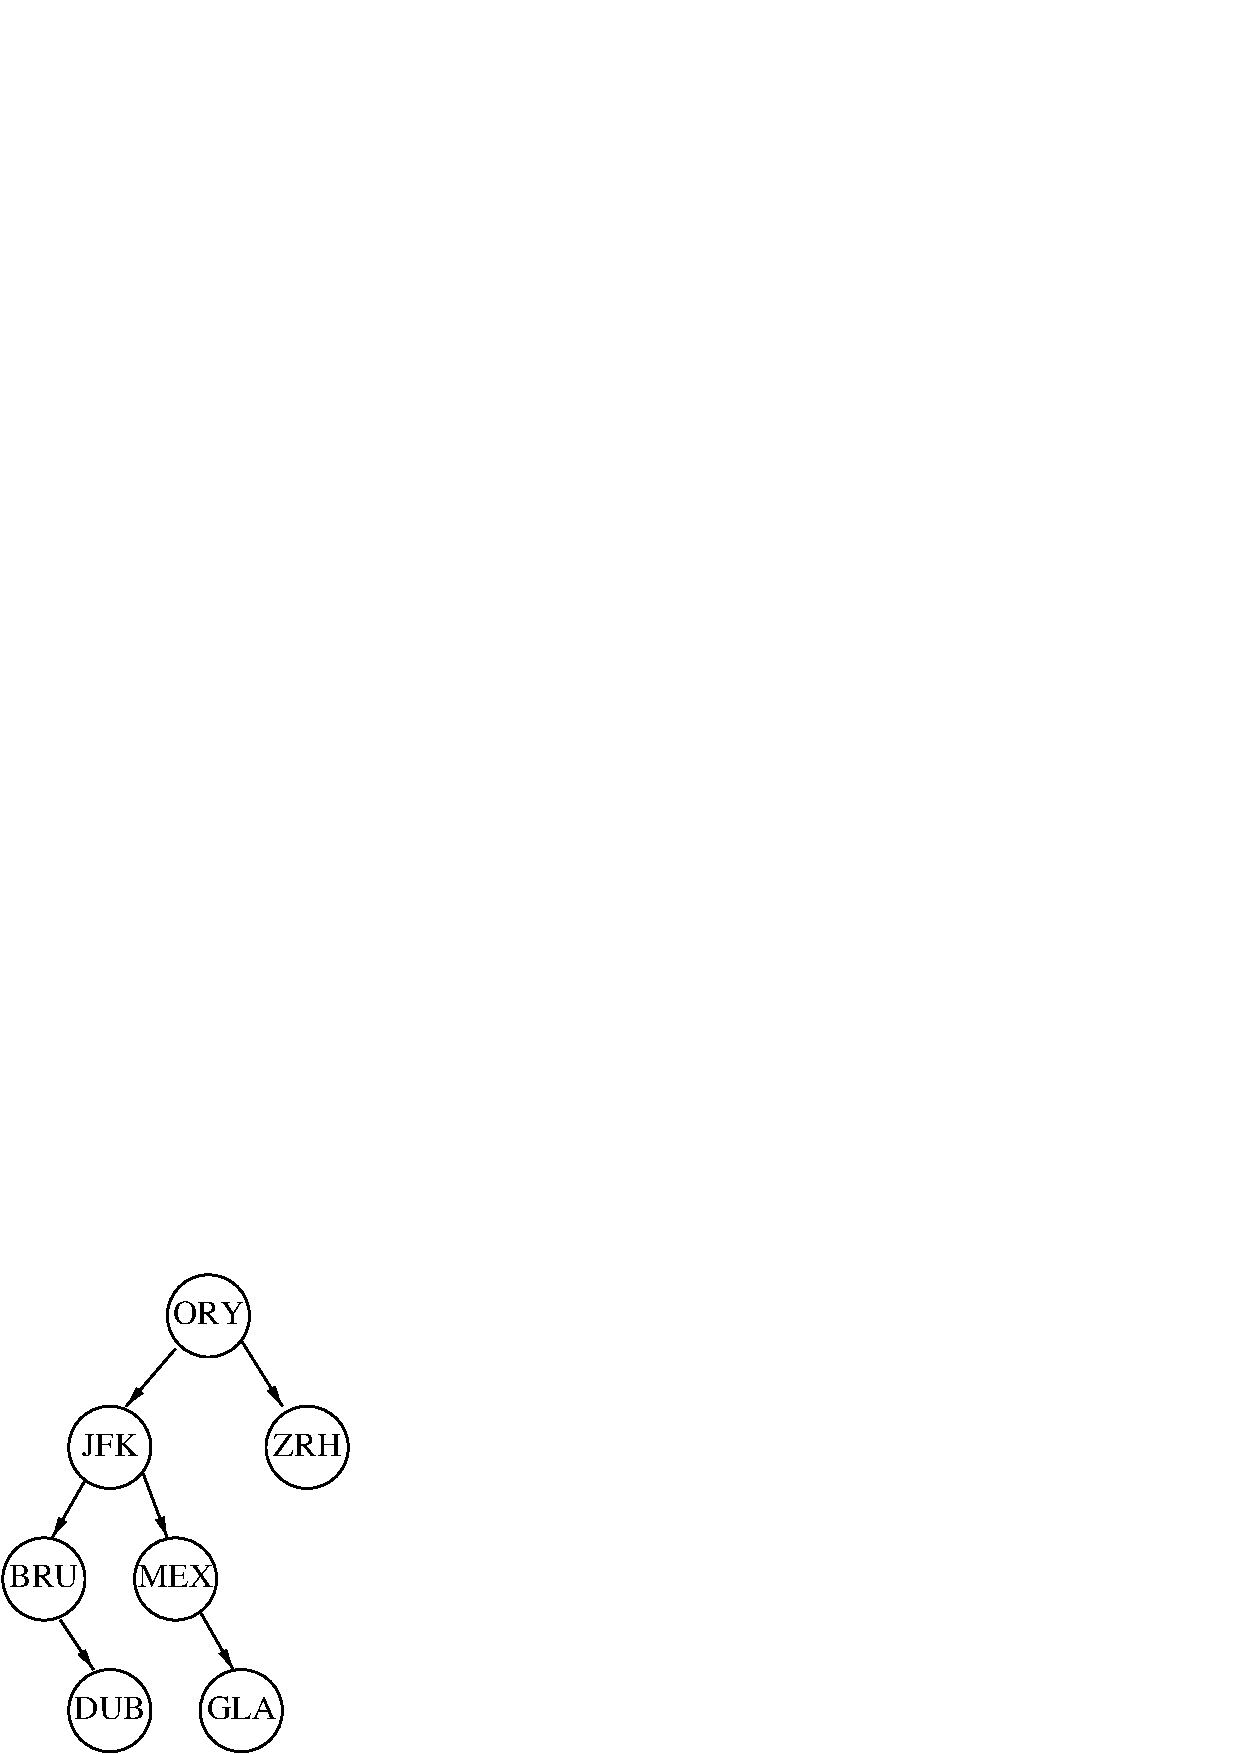
\includegraphics{../Images/treeapt.pdf}	
\end{center}	
}	

\newpage	
{\samepage	
\begin{center}	
{\Large{\bf My BST ADT}}	
\end{center}	
{\small	
\begin{verbatim}	
bst* bst_init(void);	
/* Insert 1 item into the tree */	
bool bst_insert(bst* b, datatype d);	
/* Return number of datatypes in tree */	
int bst_size(bst* b);	
/* Whether the data d is stored in the tree */	
bool bst_isin(bst* b, datatype d);	
/* Bulk insert n items from an array a into an initialised tree */	
bool bst_insertarray(bst* b, datatype* a, int n);	
/* Clear all memory associated with tree, & set pointer to NULL */	
bool bst_free(bst* b);	
/* Optional ? */	
char* bst_preorder(bst* b);	
void bst_printlevel(bst* b);	
/* Create string with tree as ((head)(left)(right)) */	
char* bst_printlisp(bst* b);	
/* Use Graphviz via a .dot file */	
void bst_todot(bst* b, char* dotname);	
\end{verbatim}	
}}	

\newpage	
{\samepage	
\begin{center}	
{\Large{\bf Binary Search Trees}}	
\end{center}	
\begin{verbatim}	
/* Based on geekforgeeks.org */	
dataframe* _insert(dataframe* t, datatype d)	
{	
    dataframe* f;	
    /* If the tree is empty, return a new frame */	
    if (t == NULL){	
       f = ncalloc(sizeof(dataframe), 1);	
       f->d = d;	
       return f;	
    }	
    /* Otherwise, recurs down the tree */	
    if (d < t->d){	
        t->left = _insert(t->left, d);	
    }	
    else if(d > t->d){	
       t->right = _insert(t->right, d);	
    }	
    /* return the (unchanged) dataframe pointer */	
    return t;	
}	
\end{verbatim}	
}	

\newpage	
{\samepage	
\begin{center}	
{\Large{\bf Binary Search Trees}}	
\end{center}	
{\small	
\begin{verbatim}	
char* _printlisp(dataframe* t)	
{	
   char tmp[ELEMSIZE];	
   char *s1, *s2, *p;	
   if(t==NULL){	
      /*  \0 string */	
      p = ncalloc(1,1);	
      return p;	
   }	
   sprintf(tmp, FORMATSTR, t->d);	
   s1 = _printlisp(t->left);	
   s2 = _printlisp(t->right);	
   p = ncalloc(strlen(s1)+strlen(s2)+strlen(tmp)+strlen("()() "), 1);	
   sprintf(p, "%s(%s)(%s)", tmp, s1, s2);	
   free(s1);	
   free(s2);	
   return p;	
}	
\end{verbatim}	
}	

\newpage	
{\samepage	
\begin{center}	
{\Large{\bf Binary Search Trees}}	
\end{center}	
\begin{verbatim}	
int InTree(Node *t, int i)	
{	
   if(t == NULL) return 0;	
   if(i == t->num) return 1;	
   if(i < t->num)	
      return InTree(t->left, i);	
   else	
      return InTree(t->right, i);	
}	
\end{verbatim}	
}	

\newpage	
{\samepage	
\begin{center}	
{\Large{\bf Level Order Traversal}}	
\end{center}	
\begin{center}	
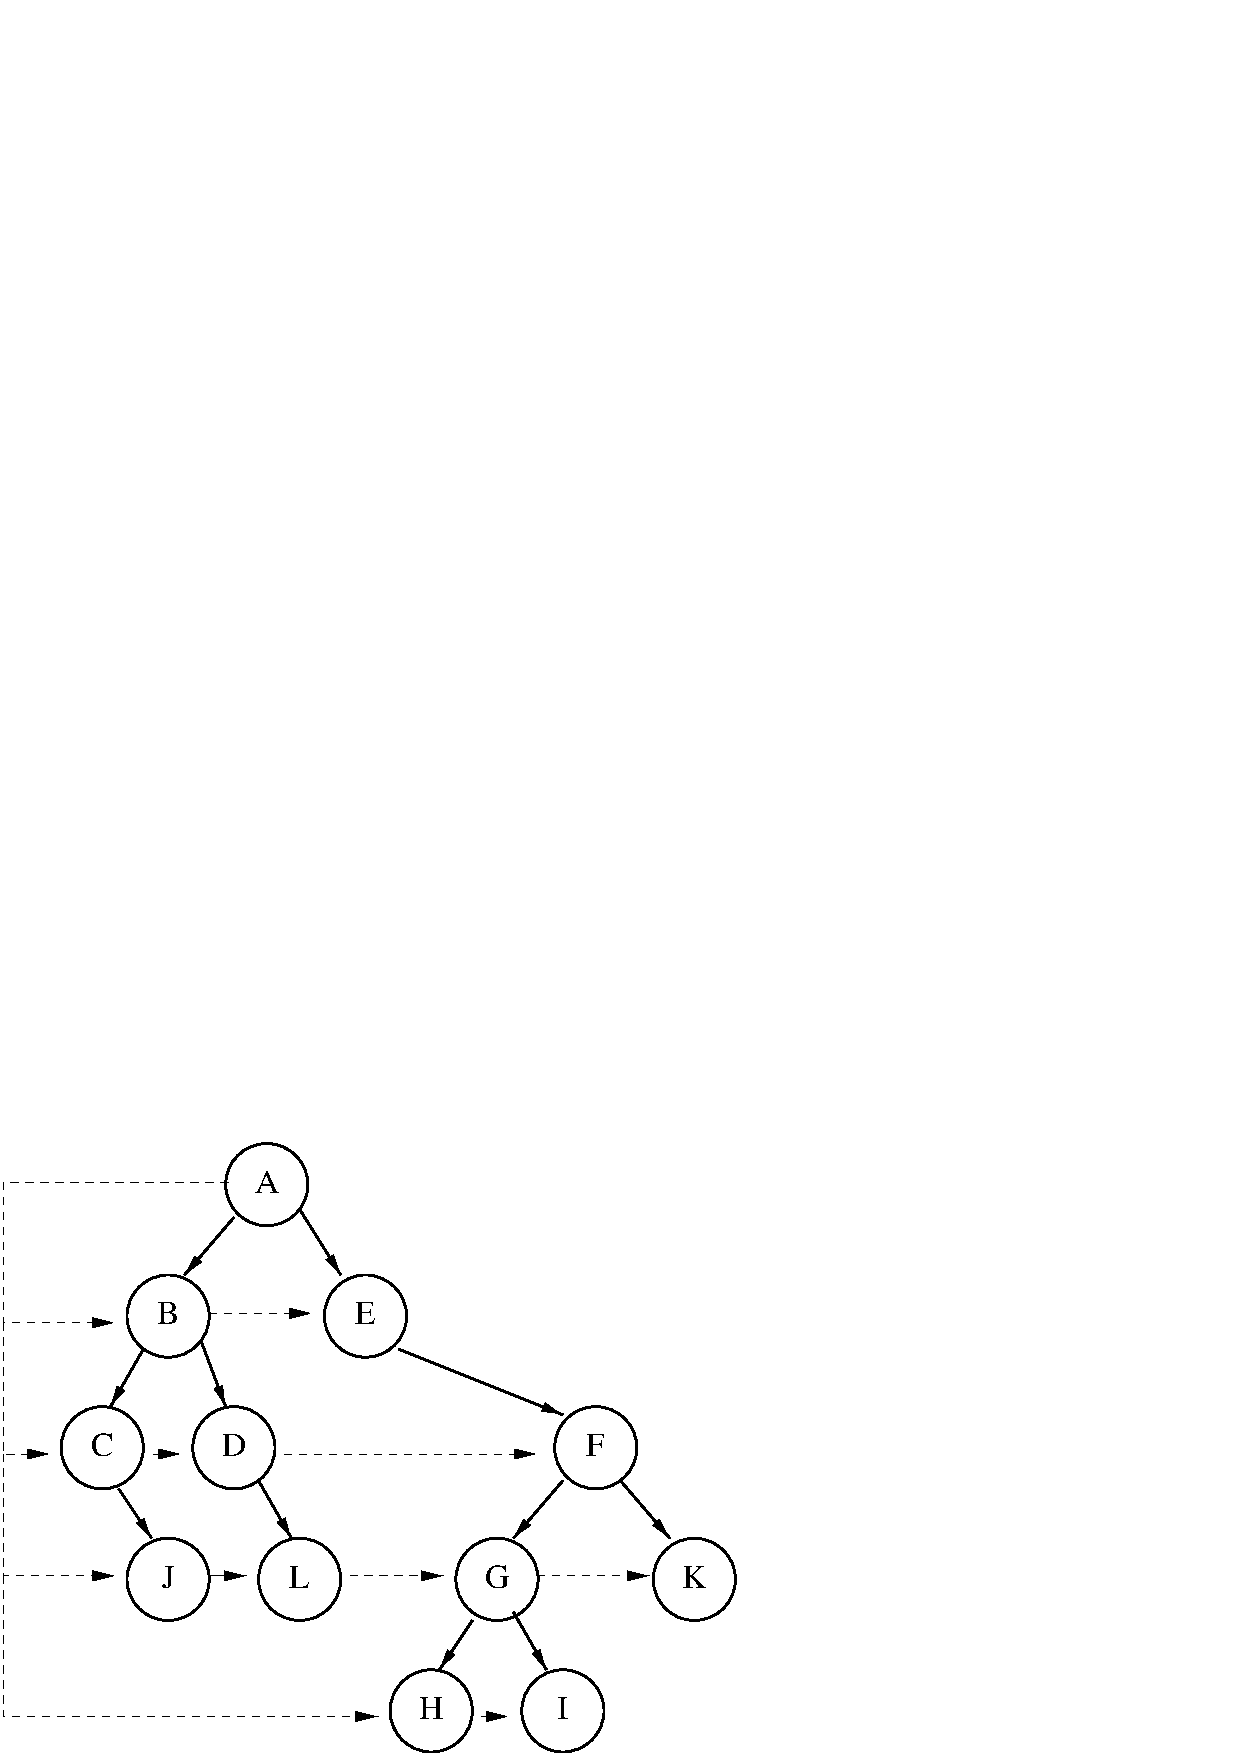
\includegraphics{../Images/treelvl.pdf}	
\end{center}	
To achieve this we need to use a Queue.	
}	

\newpage	
{\samepage	
\begin{center}	
{\Large{\bf Level Order Traversal}}	
\end{center}	
\begin{verbatim}	
void bst_printlevel(bst* b)	
{	
   datatype n;	
   queue *q;	
   if((b==NULL) || (! _isvalid(b, 0))){	
      return;	
   }	
   /* Make a queue of cell indices */	
   q = queue_init();	
   queue_enqueue(q, 0);	
   while(queue_dequeue(q, &n) &&	
         _isvalid(b, (int)n)){	
      printf(FORMATSTR, b->a[n].d);	
      putchar(' ');	
      queue_enqueue(q, _leftchild((int)n));	
      queue_enqueue(q, _rightchild((int)n));	
   }	
}	
\end{verbatim}	
}	

\newpage	
{\samepage	
\begin{center}	
{\Large{\bf Binary Search Trees}}	
\end{center}	
\begin{itemize}	
\item  If the root of the tree is not well chosen, or the keys to be inserted are ordered, the tree can become a linked list !	
\item The tree search performs best when well balanced trees are formed - large	
body of literature about creating \& re-balancing trees.	
\end{itemize}	
}	






\newpage	
{\samepage	
\begin{center}	
{\Large{\bf Huffman Compression}}	
\end{center}	
\begin{itemize}	
\item Often we wish to compress data, to reduce storage requirements, or to speed transmission.	
\item  Text is particularly suited to compression since using one byte per character is wasteful - some letters occur much more frequently.	
\item  Need to give frequently occurring letters short codes, typically a few bits. Less common letters can have long bit patterns.	
\item To encode the string "BABBAGE"	
\begin{center}	
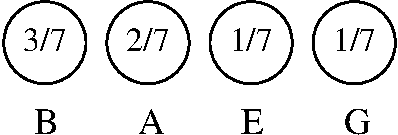
\includegraphics{../Images/huff1.pdf}	
\end{center}	
\end{itemize}	
}	

\newpage	
{\samepage	
\begin{center}	
{\Large{\bf Huffman Compression}}	
\end{center}	
{\small	
\begin{itemize}	
\item Keep a list of characters, ordered by their frequency	
\item Use the two least frequent to form a sub-tree, and re-order the nodes.	
\begin{center}	
\includegraphics{../Images/huff2.pdf}	
\end{center}	
\begin{center}	
\includegraphics{../Images/huff3.pdf}	
\end{center}	
\item A = 10, B = 0, E = 110, G = 111	
\item String stored using 13 bits.	
\end{itemize}	
}	
}	












